\documentclass{article}
\usepackage{graphicx}
\usepackage[spanish]{babel}
\usepackage{amsmath}
\usepackage{url}
\usepackage{tikz}
\usetikzlibrary{arrows.meta, positioning}
\usetikzlibrary{3d, shapes.geometric}


%%%{{{ Comments and the like
\usepackage[textwidth=4cm]{todonotes}
\usepackage{soul}
\usepackage{xcolor}
\newcounter{todocounter}
\newcommand{\comment}[2]{\stepcounter{todocounter}
  {\color{green!50!blue}{(#1$^{{\color{black}\textbf{\thetodocounter}}}$)}}
  \todo[color=green,noline,size=\tiny]{\textbf{\thetodocounter:} #2

  }}
\newcommand{\quitaesto}[1]{{\color{red}(\st{#1})}}

\newcommand{\cambio}[2]{{\color{cyan}{{#2}}}{\color{red}{(\st{#1})}}}

\newcommand{\agregaesto}[1]{{\color{cyan}{{#1}}}}

\newcommand{\notaparaelautor}[1]{{\color{brown}{\textbf{#1}}}}

\newcommand{\errorortografico}[1]{{\fcolorbox{gray}{magenta}{\textcolor{yellow}{\bf #1}}}}
    
%%%}}}

\title{Detalles de implementación}
\author{Anabel Benítez González}
\date{}

\begin{document}

% \tableofcontents
\maketitle

En este capítulo se describe una herramienta diseñada para apoyar el estudio independiente de  la asignatura Programación en \mbox{MATCOM}. La propuesta consiste en un bot de Telegram que funciona como asistente educativo interactivo, proporcionando respuestas a dudas sobre el contenido y ejercicios ajustados a las necesidades de los estudiantes. Este capítulo describe los componentes de la arquitectura del bot y sus funcionalidades principales.

\section{Selección de la plataforma: ¿Por qué Telegram?}

Telegram fue seleccionado como la plataforma para el desarrollo de la aplicación debido a varias ventajas. Su API es gratuita y está documentada, lo que facilita la implementación de funcionalidades y el desarrollo de características específicas. Asimismo, Telegram es accesible desde múltiples dispositivos, como teléfonos móviles y laptops, e incluso permite sesiones simultáneas en ambos, garantizando así una experiencia fluida, disponibilidad constante y comodidad para los estudiantes.

Otra razón importante para esta elección es que los estudiantes de la facultad ya están familiarizados con Telegram desde el primer año de la carrera, ya que la aplicación se utiliza ampliamente como herramienta de comunicación en MATCOM. Esto elimina la necesidad de aprender a manejar una nueva herramienta o de incorporar otra aplicación a su rutina, evitando distracciones adicionales. El bot propuesto simplemente se integra como un nuevo chat en una plataforma que los estudiantes ya utilizan con regularidad.

% \section{Descripción de la aplicación propuesta}

% El objetivo del bot es mejorar la experiencia de estudio independiente de los estudiantes de Programación. Para ello, combina un conjunto de funcionalidades diseñadas para facilitar el aprendizaje y fomentar la autonomía:

% \subsection{Resolución de dudas}

% Resolución de dudas: Los estudiantes pueden formular preguntas relacionadas con conceptos de programación utilizando lenguaje natural. El bot responde con explicaciones claras y referencias a la bibliografía oficial de la asignatura.

% \textit{/ask [tema o duda específica]}:  
%     Permite a los estudiantes realizar preguntas relacionadas con conceptos de programación.
    
% \subsection{Listado de temas}

% \textit{/topics}:  
%     Lista los temas disponibles para explorar nuevos contenidos de estudio.

% \subsection{Sugerencia de ejercicios}
% Sugerencia de ejercicios: Se analiza el historial de ejercicios realizados por el estudiante y se proponen ejercicios acordes al nivel del estudiante, intentando garantizar un aprendizaje progresivo.

% \textit{/exercise [tema]}:  
%     Sugiere ejercicios en función del progreso del estudiante.

% \subsection{Recomendación de pistas}

% Recomendación de pistas: Cada ejercicio incluye un sistema de pistas escalonadas que fomenta la autonomía del estudiante. Estas pistas aportan ayuda para resolver el ejercicio sin ofrecer directamente la solución.

% \textit{/hint [número de ejercicio]}:  
%     Proporciona pistas escalonadas para un ejercicio específico.

% \subsection{Otros comandos}
% \textit{/start}:  
%     Inicia la interacción con el bot. Guarda al estudiante en el sistema y muestra un mensaje de bienvenida y una guía básica sobre cómo usar las funcionalidades disponibles.
    
% \textit{/help}:  
%     Muestra una lista de todos los comandos disponibles junto con una breve descripción de cada uno. Es útil para estudiantes que necesitan orientación rápida sobre cómo interactuar con el bot.  

\section{Arquitectura y componentes principales}

En las siguientes secciones, se profundiza en el funcionamiento interno de los principales componentes del bot.

\subsection{Resolución de dudas}

El diagrama de la Figura~\ref{fig:q-a-diagram} ilustra cómo se utiliza el sistema basado en Generación Aumentada por Recuperación (RAG) para resolver las dudas de los estudiantes.

Como se explica en el Capítulo~\ref{chapter:rag} el proceso de construcción del recuperador consta de tres etapas: dividir el corpus en fragmentos, codificar los fragmentos y construir la base de datos vectorial.

El corpus del sistema está compuesto por los capítulos del libro ``Empezar a programar: Un enfoque multiparadigma con C\#'' en formato PDF. Este contenido se convierte a texto utilizando herramientas de extracción que preservan su estructura original. Para manejar el contenido, se divide en fragmentos de longitud fija de 2000 caracteres con un solapamiento de 200 caracteres, lo que garantiza que no se pierda el contexto entre fragmentos consecutivos. Cada fragmento se transforma en una representación numérica mediante el modelo de embeddings \textit{models/text-embedding-004} de Google.

Durante este proceso, a cada fragmento se le asocian metadatos, como el nombre del documento y el número de página correspondiente. Estos metadatos se almacenan junto con los vectores en la base de datos vectorial, lo que permite, durante la fase de generación, incorporar referencias en las respuestas proporcionadas al usuario.

Cuando un estudiante formula una pregunta, esta se procesa mediante el mismo modelo \textit{models/text-embedding-004}, que convierte la pregunta en una representación vectorial. Para medir la relevancia entre una consulta y los fragmentos almacenados en la base de datos vectorial, se emplea la similitud coseno. El sistema utiliza los 5 fragmentos más similares para generar el \textit{prompt} extendido, que combina la pregunta con el contenido relevante del libro.

El \textit{prompt} extendido se envía al LLM \textit{gemini-1.5-flash}, que genera una respuesta detallada. Además, las respuestas están enriquecidas con referencias específicas al libro, permitiendo al estudiante verificar la información en una fuente confiable.

Este flujo de trabajo muestra cómo el sistema RAG integra la búsqueda de información con la generación de texto, reduciendo el tiempo que el estudiante dedicaría a buscar respuestas por otros medios, como el libro o la consulta directa al profesor. Al incluir referencias al libro de Katrib, el sistema permite al estudiante verificar la información directamente en una fuente confiable, evitando la dependencia exclusiva LLMs o fuentes en línea que podrían no ser fiables, especialmente para estudiantes inexpertos. Este enfoque busca no solo fomentar la autonomía del estudiante, sino también reforzar su capacidad para validar la información de manera independiente.

\begin{figure}[h!]
    \centering
    \begin{tikzpicture}[
      font=\sffamily,
      every node/.style={align=center},
      box/.style={draw, rectangle, minimum width=3cm, minimum height=1cm},
      arrow/.style={-Latex},
      db/.style={cylinder, cylinder uses custom fill, cylinder body fill=blue!20, shape border rotate=90, aspect=0.25, minimum height=1.5cm, minimum width=1cm, draw}
    ]
    
    \node[box] (materials) {Libro de Katrib};
    \node[box, below=1cm of materials] (question) {Pregunta};
    \node[box, right=0.8cm of question] (embedding) {Función \\de \\Embedding};
    \node[db, right=2cm of embedding] (database) {Base de Datos \\Vectorial};
    \node[box, below=2.5cm of database] (prompt) {Prompt Extendido = \\Pregunta +\\Contenido del libro};
    \node[box, below=1.5cm of prompt] (llm) {LLM};
    % \node[box, left=2.5cm of llm] (professor) {Profesor};
    \node[box, left=2.5cm of llm] (reply) {Respuesta \\con referencias al libro};
    \node[below=1.5cm of question] (user) {
      \begin{tikzpicture}[scale=0.8] % Escala más grande
        % Cabeza
        \draw (0,0.7) circle [radius=0.3]; % Cabeza más grande y sin relleno
        % Cuerpo
        \draw (0,0.4) -- (0,-0.5); % Línea del cuerpo
        \draw (-0.4,-1) -- (0,-0.5) -- (0.4,-1); % Piernas
        \draw (-0.3,-0.2) -- (0,0.2) -- (0.3,-0.2); % Brazos
      \end{tikzpicture}
      \\ Estudiante
    };
    
    % Arrows
    \draw[arrow] (materials) -- (embedding);
    \draw[arrow] (user) -- (question);
    \draw[arrow] (question) -- (embedding);
    % \draw[arrow] (embedding) -- node[above] {Guardar} (database);
    % Two distinct arrows between nodes
    \draw[arrow, bend left=15] (embedding) to node[above] {Guardar} (database);
    \draw[arrow, bend right=15] (embedding) to node[below] {Búsqueda \\por \\similitud} (database);
    
    \draw[arrow] (database) -- node[right] {Fragmentos \\recuperados} (prompt);
    \draw[arrow] (prompt) -- (llm);
    \draw[arrow] (llm) -- (reply);
    \draw[arrow] (reply) -- ++(0,1) -| (user);
    
    \end{tikzpicture}
    \caption{Diagrama de flujo del sistema de preguntas y respuestas basado en Generación Aumentada por Recuperación (RAG)}\label{fig:q-a-diagram}
\end{figure}


\subsection{Recomendación de ejercicios y pistas}

El diseño del sistema facilita la integración de nuevos temas, ejercicios y pistas, estos son extraídos de un archivo json, cuyo formato está descrito en el repositorio de Github.

El sistema de ejercicios y pistas está diseñado para ofrecer a los estudiantes una experiencia de aprendizaje adaptada a su ritmo y necesidades. Los estudiantes pueden avanzar de forma independiente resolviendo ejercicios, con la opción de solicitar pistas cuando enfrentan dificultades.

Los ejercicios están organizados por temas, como condicionales o arrays, y clasificados en niveles de dificultad: básico, intermedio y avanzado. Esta organización permite recomendar ejercicios que ayuden a los estudiantes a avanzar paso a paso y a concentrarse en los temas que más necesitan o les interesan, intentando evitar la sobrecarga cognitiva.

Cada estudiante tiene un estado asociado a cada ejercicio, que puede ser ``En Progreso'', ``Enviado'' o ``Completado''. Este sistema de seguimiento permite monitorear el avance individual y utilizar el historial de ejercicios para recomendar nuevos problemas al estudiante, considerando los temas ya dominados y las áreas que aún necesita reforzar.


El sistema de pistas está diseñado para acompañar a los estudiantes en la resolución de ejercicios mediante apoyo gradual. Cada ejercicio dispone de una serie de pistas organizadas en niveles, que los estudiantes pueden solicitar según lo necesiten. Las pistas se entregan de manera progresiva, comenzando con consejos generales y avanzando hacia indicaciones más específicas. Actualmente, este sistema solo está disponible para ejercicios relacionados con arrays, pero puede ampliarse fácilmente a otros temas al agregar las pistas correspondientes a cada ejercicio a la base de datos.

Además, cada vez que un estudiante solicita una pista, el sistema registra esta acción, creando un historial detallado. Este registro permite analizar el uso de las pistas, identificar patrones de dependencia y evaluar cómo progresa cada estudiante en la resolución de problemas de manera autónoma.\\

\begin{figure}
    \centering
    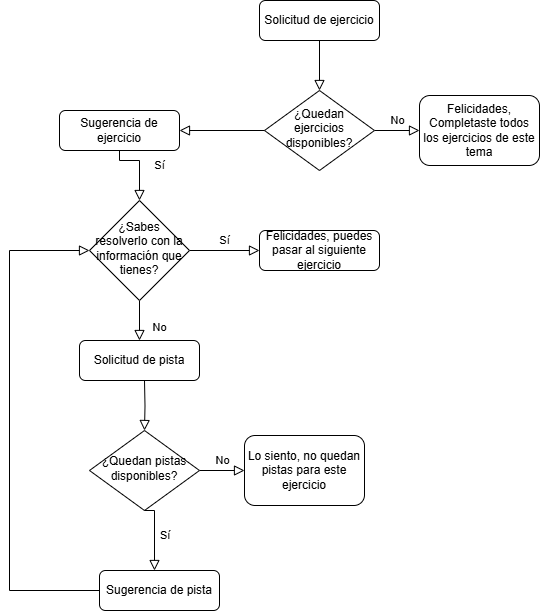
\includegraphics[width=0.7\linewidth]{flow.png}
    \caption{Diagrama de flujo del sistema de ejercicios y pistas}
    \label{fig:e-h-diagram}
\end{figure}

El bot tiene el potencial de impactar positivamente la enseñanza de Programación. Su diseño permite personalizar el aprendizaje según las necesidades individuales de cada estudiante, recomendando ejercicios adecuados a su nivel y brindando pistas progresivas, en caso de que las necesiten. Además, al ofrecer respuestas claras y referencias confiables, podría facilitar una mejor comprensión de los conceptos clave de programación.

Al estar implementado en una plataforma como Telegram, el bot sería fácilmente accesible para los estudiantes, quienes podrían usarlo en cualquier momento y desde cualquier dispositivo. Esto fomentaría un aprendizaje flexible y autodirigido, eliminando barreras de acceso a los recursos educativos.

El enfoque del bot también promovería la autonomía. Las pistas progresivas están pensadas para motivar a los estudiantes a resolver problemas por sí mismos, desarrollando habilidades importantes como el pensamiento lógico y la resolución de problemas. De forma complementaria, el monitoreo del progreso permite ajustar recomendaciones de ejercicios y pistas, adaptándose continuamente a las necesidades del estudiante.

% \begin{thebibliography}{99}
% \end{thebibliography}

\end{document}